% Options for packages loaded elsewhere
\PassOptionsToPackage{unicode}{hyperref}
\PassOptionsToPackage{hyphens}{url}
%
\documentclass[
]{article}
\usepackage{lmodern}
\usepackage{amssymb,amsmath}
\usepackage{ifxetex,ifluatex}
\ifnum 0\ifxetex 1\fi\ifluatex 1\fi=0 % if pdftex
  \usepackage[T1]{fontenc}
  \usepackage[utf8]{inputenc}
  \usepackage{textcomp} % provide euro and other symbols
\else % if luatex or xetex
  \usepackage{unicode-math}
  \defaultfontfeatures{Scale=MatchLowercase}
  \defaultfontfeatures[\rmfamily]{Ligatures=TeX,Scale=1}
\fi
% Use upquote if available, for straight quotes in verbatim environments
\IfFileExists{upquote.sty}{\usepackage{upquote}}{}
\IfFileExists{microtype.sty}{% use microtype if available
  \usepackage[]{microtype}
  \UseMicrotypeSet[protrusion]{basicmath} % disable protrusion for tt fonts
}{}
\makeatletter
\@ifundefined{KOMAClassName}{% if non-KOMA class
  \IfFileExists{parskip.sty}{%
    \usepackage{parskip}
  }{% else
    \setlength{\parindent}{0pt}
    \setlength{\parskip}{6pt plus 2pt minus 1pt}}
}{% if KOMA class
  \KOMAoptions{parskip=half}}
\makeatother
\usepackage{xcolor}
\IfFileExists{xurl.sty}{\usepackage{xurl}}{} % add URL line breaks if available
\IfFileExists{bookmark.sty}{\usepackage{bookmark}}{\usepackage{hyperref}}
\hypersetup{
  pdftitle={Impulsivity,Alcohol Use, and Frequency of Bullying victimization as Predictors for Coexisting Bullying Perpetration among Taiwanese Adolescents},
  pdfauthor={Tzu-Hsien Liao1, Kuo-Yang Huang2, Shen-Ing Liu 1,3*},
  hidelinks,
  pdfcreator={LaTeX via pandoc}}
\urlstyle{same} % disable monospaced font for URLs
\usepackage[margin=1in]{geometry}
\usepackage{color}
\usepackage{fancyvrb}
\newcommand{\VerbBar}{|}
\newcommand{\VERB}{\Verb[commandchars=\\\{\}]}
\DefineVerbatimEnvironment{Highlighting}{Verbatim}{commandchars=\\\{\}}
% Add ',fontsize=\small' for more characters per line
\usepackage{framed}
\definecolor{shadecolor}{RGB}{248,248,248}
\newenvironment{Shaded}{\begin{snugshade}}{\end{snugshade}}
\newcommand{\AlertTok}[1]{\textcolor[rgb]{0.94,0.16,0.16}{#1}}
\newcommand{\AnnotationTok}[1]{\textcolor[rgb]{0.56,0.35,0.01}{\textbf{\textit{#1}}}}
\newcommand{\AttributeTok}[1]{\textcolor[rgb]{0.77,0.63,0.00}{#1}}
\newcommand{\BaseNTok}[1]{\textcolor[rgb]{0.00,0.00,0.81}{#1}}
\newcommand{\BuiltInTok}[1]{#1}
\newcommand{\CharTok}[1]{\textcolor[rgb]{0.31,0.60,0.02}{#1}}
\newcommand{\CommentTok}[1]{\textcolor[rgb]{0.56,0.35,0.01}{\textit{#1}}}
\newcommand{\CommentVarTok}[1]{\textcolor[rgb]{0.56,0.35,0.01}{\textbf{\textit{#1}}}}
\newcommand{\ConstantTok}[1]{\textcolor[rgb]{0.00,0.00,0.00}{#1}}
\newcommand{\ControlFlowTok}[1]{\textcolor[rgb]{0.13,0.29,0.53}{\textbf{#1}}}
\newcommand{\DataTypeTok}[1]{\textcolor[rgb]{0.13,0.29,0.53}{#1}}
\newcommand{\DecValTok}[1]{\textcolor[rgb]{0.00,0.00,0.81}{#1}}
\newcommand{\DocumentationTok}[1]{\textcolor[rgb]{0.56,0.35,0.01}{\textbf{\textit{#1}}}}
\newcommand{\ErrorTok}[1]{\textcolor[rgb]{0.64,0.00,0.00}{\textbf{#1}}}
\newcommand{\ExtensionTok}[1]{#1}
\newcommand{\FloatTok}[1]{\textcolor[rgb]{0.00,0.00,0.81}{#1}}
\newcommand{\FunctionTok}[1]{\textcolor[rgb]{0.00,0.00,0.00}{#1}}
\newcommand{\ImportTok}[1]{#1}
\newcommand{\InformationTok}[1]{\textcolor[rgb]{0.56,0.35,0.01}{\textbf{\textit{#1}}}}
\newcommand{\KeywordTok}[1]{\textcolor[rgb]{0.13,0.29,0.53}{\textbf{#1}}}
\newcommand{\NormalTok}[1]{#1}
\newcommand{\OperatorTok}[1]{\textcolor[rgb]{0.81,0.36,0.00}{\textbf{#1}}}
\newcommand{\OtherTok}[1]{\textcolor[rgb]{0.56,0.35,0.01}{#1}}
\newcommand{\PreprocessorTok}[1]{\textcolor[rgb]{0.56,0.35,0.01}{\textit{#1}}}
\newcommand{\RegionMarkerTok}[1]{#1}
\newcommand{\SpecialCharTok}[1]{\textcolor[rgb]{0.00,0.00,0.00}{#1}}
\newcommand{\SpecialStringTok}[1]{\textcolor[rgb]{0.31,0.60,0.02}{#1}}
\newcommand{\StringTok}[1]{\textcolor[rgb]{0.31,0.60,0.02}{#1}}
\newcommand{\VariableTok}[1]{\textcolor[rgb]{0.00,0.00,0.00}{#1}}
\newcommand{\VerbatimStringTok}[1]{\textcolor[rgb]{0.31,0.60,0.02}{#1}}
\newcommand{\WarningTok}[1]{\textcolor[rgb]{0.56,0.35,0.01}{\textbf{\textit{#1}}}}
\usepackage{graphicx,grffile}
\makeatletter
\def\maxwidth{\ifdim\Gin@nat@width>\linewidth\linewidth\else\Gin@nat@width\fi}
\def\maxheight{\ifdim\Gin@nat@height>\textheight\textheight\else\Gin@nat@height\fi}
\makeatother
% Scale images if necessary, so that they will not overflow the page
% margins by default, and it is still possible to overwrite the defaults
% using explicit options in \includegraphics[width, height, ...]{}
\setkeys{Gin}{width=\maxwidth,height=\maxheight,keepaspectratio}
% Set default figure placement to htbp
\makeatletter
\def\fps@figure{htbp}
\makeatother
\setlength{\emergencystretch}{3em} % prevent overfull lines
\providecommand{\tightlist}{%
  \setlength{\itemsep}{0pt}\setlength{\parskip}{0pt}}
\setcounter{secnumdepth}{-\maxdimen} % remove section numbering

\title{Impulsivity,Alcohol Use, and Frequency of Bullying victimization as
Predictors for Coexisting Bullying Perpetration among Taiwanese
Adolescents}
\author{Tzu-Hsien Liao1, Kuo-Yang Huang2, Shen-Ing Liu 1,3*}
\date{2020/5/12}

\begin{document}
\maketitle

\hypertarget{r-markdown}{%
\subsection{R Markdown}\label{r-markdown}}

Results

Descriptive statistics and Data Visualization

Among 733 students, 363 (49.5\%) were male, and the median/mean age at
the first evaluation was 16.38 years (SD .50). The proportions of the
bully group (the pure bully group and the bully-victim group) and the
victim group( the pure victim group and the bully-victim group) were
27.0\%( 198/733) and 37.8\%( 277/733) respectively. The proportions of
four mutually exclusive group of bullying involvement were 53.9\% ( the
not-involved group), 19.1\%( the pure victim group), 18.7\%( the
bully-victim group) and 8.3\%( the pure bully group) respectively during
the last six months( See figure 1.)
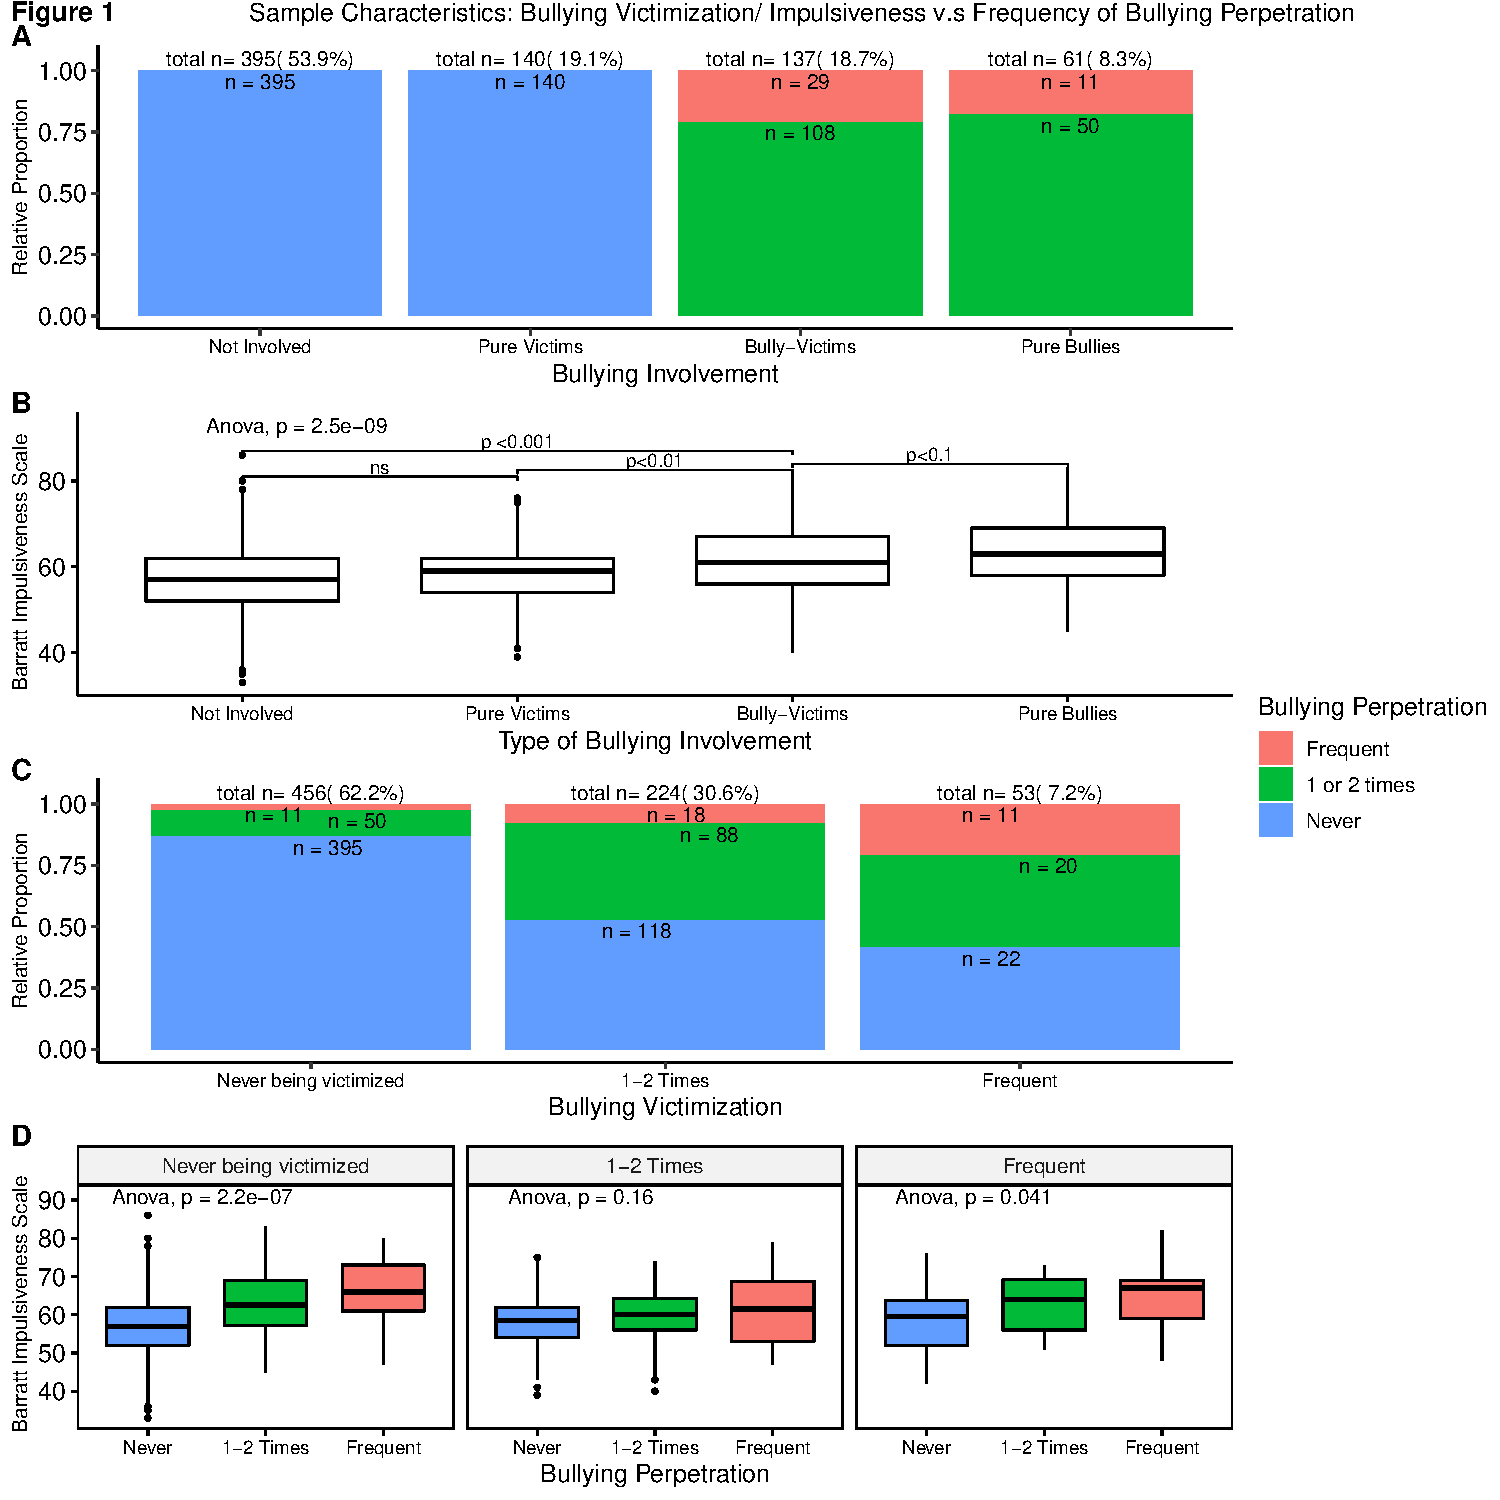
\includegraphics{Manuscript_files/figure-latex/Figure 1.-1.pdf} The
frequency of bullying perpetration increased with the frequency of
bullying victimization. The BIS of the pure bully group was
significantly higher than the bully-victim group, which also has higher
BIS than the victim group and the not-involved group with statistical
significance. The tendency of higher BIS for more frequent bullying
perpetration could also be noted when the bully group was subgrouped by
different frequency of victimization. (figure 1)

The detailed statistical summary and pairwise comparison among the
categorical and numeric variables were listed according to various
levels of bullying involvement(figure S1.1-S1.2) and frequency of
bullying perpetration(figure S2.1-S2.2).The distributions of types of
bullying involvement and sociodemographic variables, except gender(
male: female 49.5\% vs.~50.5\%), were imbalanced( figure S1,1).

\begin{Shaded}
\begin{Highlighting}[]
\KeywordTok{print}\NormalTok{(fig_s1_revised) }
\end{Highlighting}
\end{Shaded}

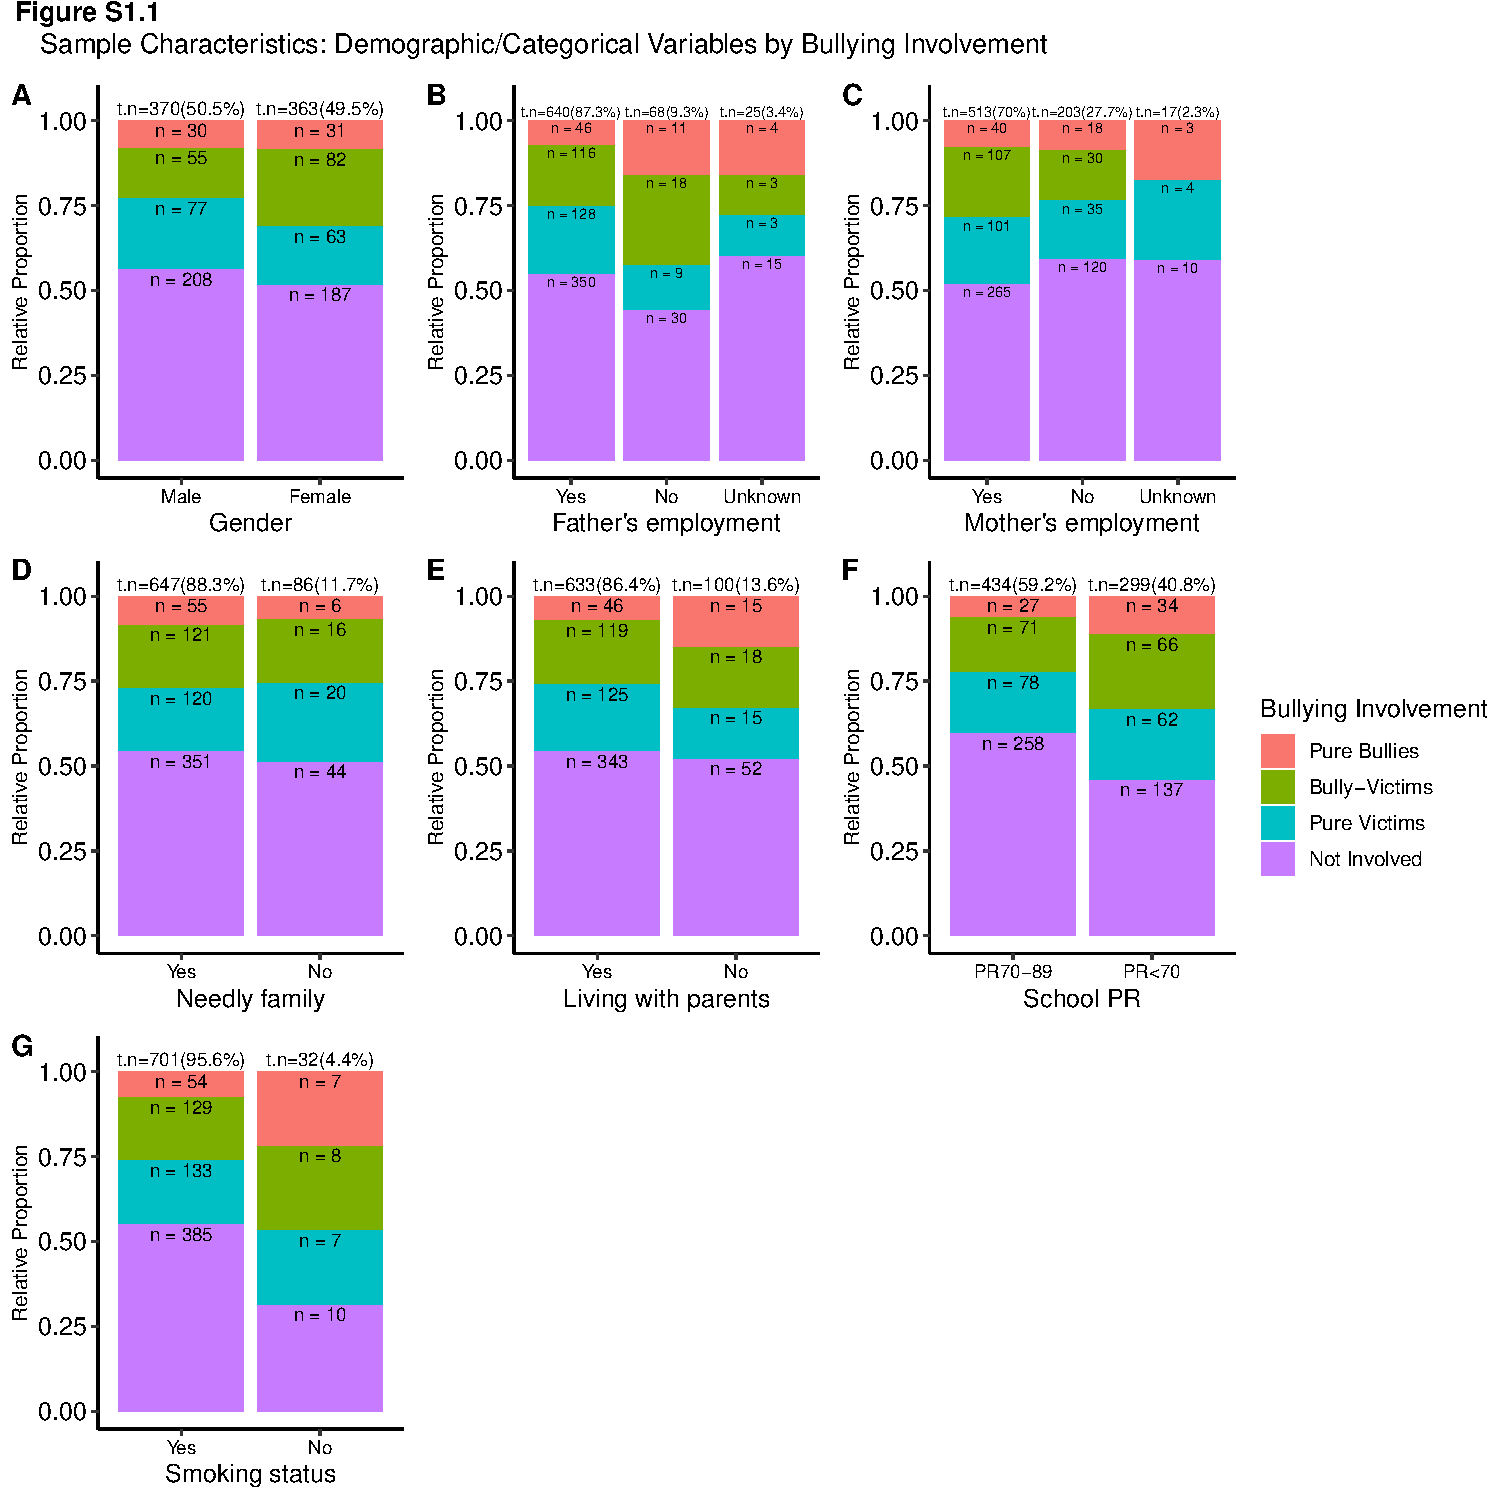
\includegraphics{Manuscript_files/figure-latex/unnamed-chunk-1-1.pdf}

The distribution imbalance of variables necessitated the use of
penalized likelihood-based method of logistic regression, such as Firth
logistic regression, in the following multivariate analyses. Most
participants had non-needy families and lived with their parents, while
their parents were mostly employed. The correlations between variables,
such as PHQ-9 and RSES, raised our concern for possible multilinearity
in multivariate analyses of these variables.

\begin{Shaded}
\begin{Highlighting}[]
\NormalTok{fig_s1_}\DecValTok{2}
\end{Highlighting}
\end{Shaded}

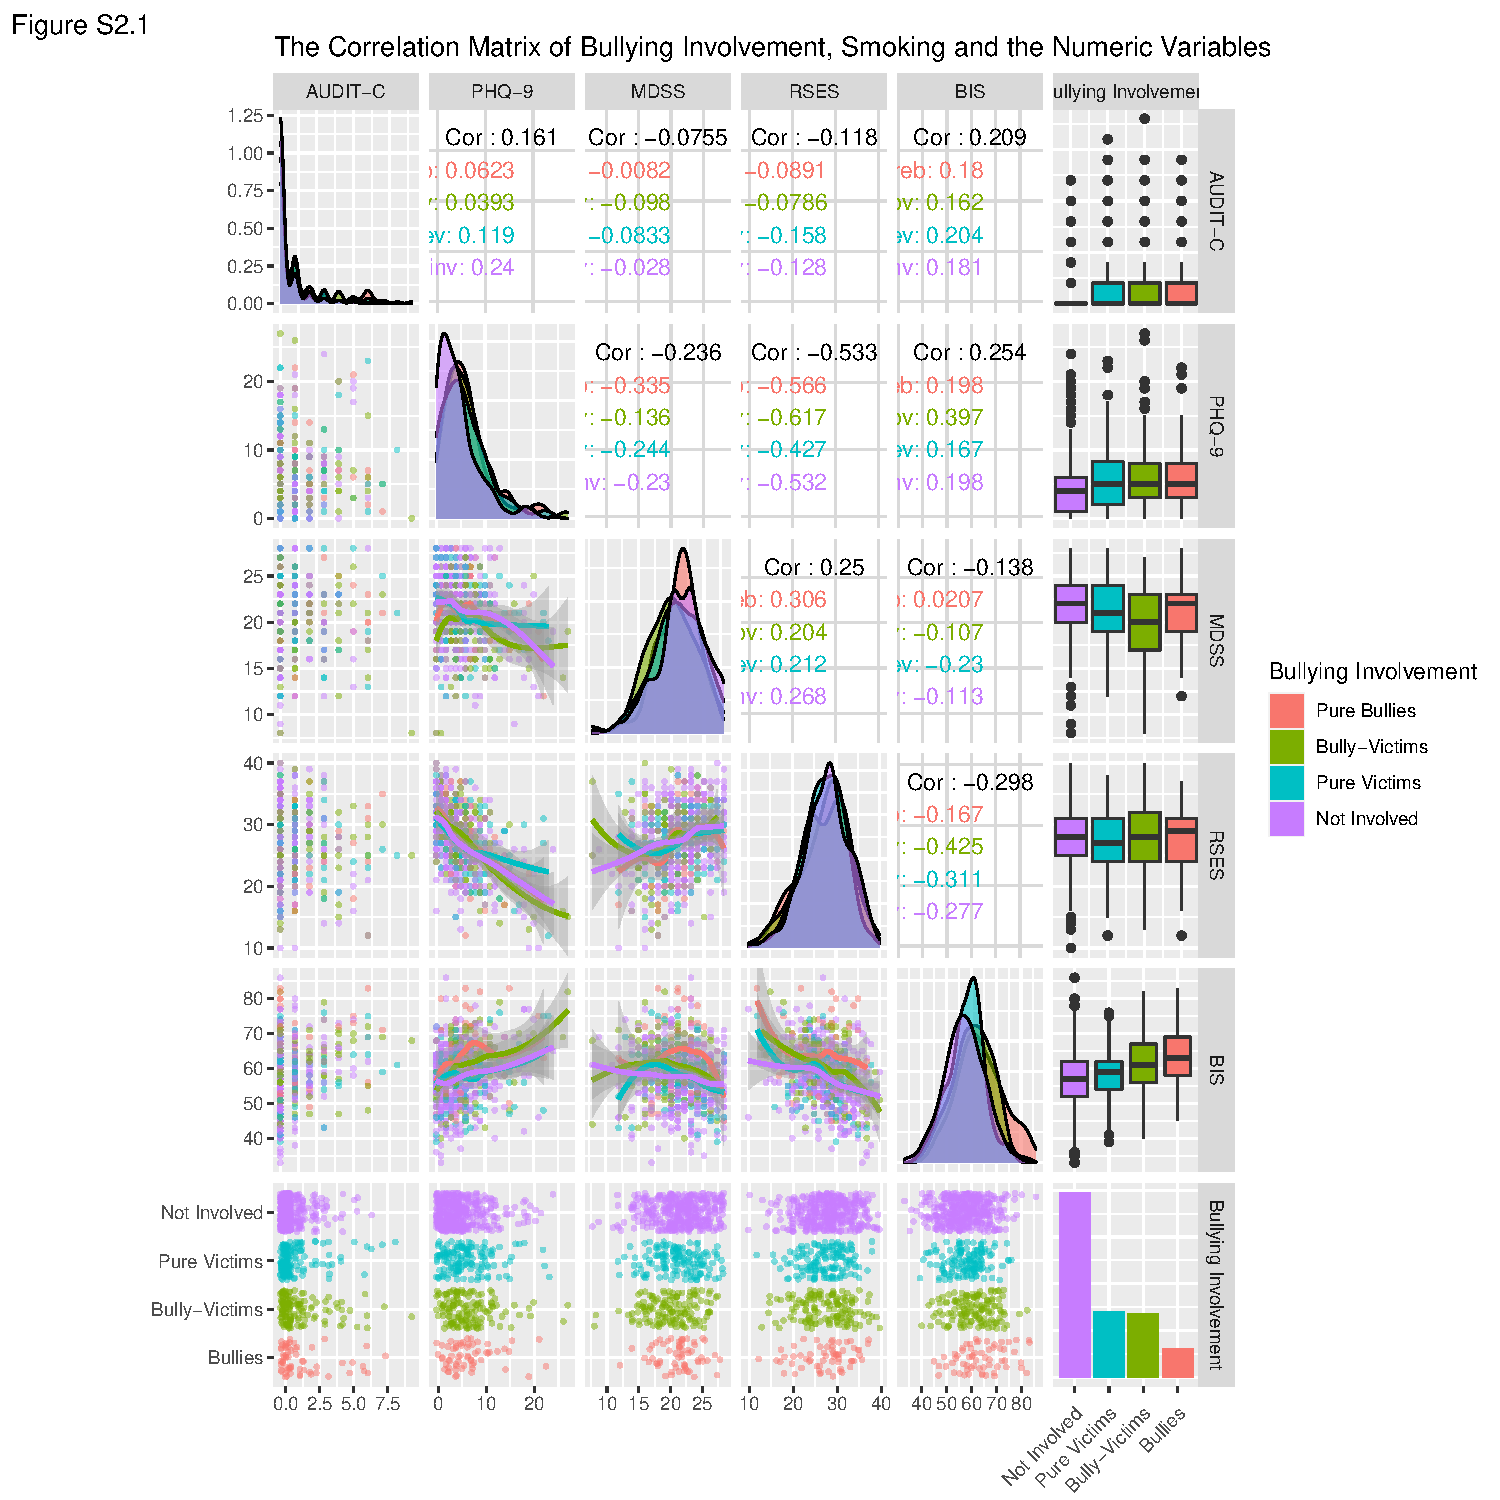
\includegraphics{Manuscript_files/figure-latex/unnamed-chunk-2-1.pdf}

Univariate Analysis: Variables associated with different involvement of
bullying perpetration

In the univariate analysis, male, school ranking≦70, father's
unemployment, smoking behavior, mild depression(scores of PHQ-9: 6 to
10,), problem drinkers( AUDIT-C ≥ 4), and higher impulsivity(higher
scores of the BIS-11) were significantly associated with the bully
group, the bully-victim group, and the frequent bully group, when
compared with the noninvolved group. (see table 2.)

\begin{Shaded}
\begin{Highlighting}[]
\KeywordTok{print}\NormalTok{(}\KeywordTok{cbind}\NormalTok{(table2}\OperatorTok{$}\NormalTok{bullies[[}\DecValTok{1}\NormalTok{]], }\DataTypeTok{Bullies =}\NormalTok{table2}\OperatorTok{$}\NormalTok{bullies[[}\DecValTok{2}\NormalTok{]],  }\DataTypeTok{Bully_victims=}\NormalTok{table2}\OperatorTok{$}\NormalTok{bully_victims[[}\DecValTok{1}\NormalTok{]], }\DataTypeTok{Pure_Bullies=}\NormalTok{ table2}\OperatorTok{$}\NormalTok{pure_bullies[[}\DecValTok{1}\NormalTok{]], }\DataTypeTok{Frequent_bullies=}\NormalTok{table2}\OperatorTok{$}\NormalTok{repeated_bullies[[}\DecValTok{1}\NormalTok{]]))}
\end{Highlighting}
\end{Shaded}

\begin{verbatim}
##                                Bullies              Bully_victims       
##  [1,] "q3_a男"                 "1.38(1.03-1.85)*"   "1.47(1.08-2)*"     
##  [2,] "school_PRPR<70"         "1.73(1.28-2.32)***" "1.53(1.12-2.09)**" 
##  [3,] "q8_a否"                 "1.16(0.87-1.56)"    "1(0.73-1.36)"      
##  [4,] "q7_a是"                 "1(0.75-1.34)"       "1(0.74-1.36)"      
##  [5,] "q6_a沒有"               "1.26(0.94-1.7)"     "1.36(1-1.86)"      
##  [6,] "q5_a沒有"               "1.48(1.09-1.99)*"   "1.32(0.96-1.81)"   
##  [7,] "q68_a是"                "1.49(1.11-2)**"     "1.28(0.94-1.74)"   
##  [8,] "PHQ9_1yr_new6-10"       "1.88(1.37-2.58)***" "1.81(1.3-2.52)***" 
##  [9,] "PHQ9_1yr_new11-14"      "1.49(1.05-2.11)*"   "1.56(1.08-2.25)*"  
## [10,] "PHQ9_1yr_new15以上"     "1.44(1.01-2.05)*"   "1.31(0.9-1.89)"    
## [11,] "AUDIT_C_4_a>=4"         "1.94(1.44-2.6)***"  "1.8(1.32-2.46)***" 
## [12,] "q22_0_a"                "0.56(0.41-0.77)***" "0.47(0.33-0.68)***"
## [13,] "firstrses_standardized" "0.84(0.62-1.15)"    "0.84(0.59-1.2)"    
## [14,] "bis1_standardized"      "2.55(1.86-3.49)***" "2.1(1.47-3)***"    
##       Pure_Bullies         Frequent_bullies   
##  [1,] "1.06(0.76-1.49)"    "1.5(1.12-2.01)**" 
##  [2,] "1.68(1.2-2.35)**"   "1.32(0.98-1.76)"  
##  [3,] "1.44(1.03-2.02)*"   "1.09(0.81-1.46)"  
##  [4,] "1.01(0.73-1.41)"    "1.08(0.8-1.44)"   
##  [5,] "1(0.71-1.4)"        "1(0.74-1.34)"     
##  [6,] "1.55(1.1-2.18)*"    "1.21(0.9-1.64)"   
##  [7,] "1.69(1.21-2.37)**"  "1.25(0.93-1.67)"  
##  [8,] "1.54(1.08-2.2)*"    "1.01(0.74-1.38)"  
##  [9,] "1.1(0.75-1.62)"     "1(0.71-1.41)"     
## [10,] "1.39(0.94-2.06)"    "1.1(0.77-1.56)"   
## [11,] "1.93(1.37-2.7)***"  "1.63(1.21-2.19)**"
## [12,] "0.83(0.51-1.36)"    "0.56(0.31-1.01)"  
## [13,] "0.84(0.52-1.37)"    "0.9(0.5-1.61)"    
## [14,] "4.01(2.44-6.59)***" "2.8(1.56-5.02)***"
\end{verbatim}

Figure S3 gives the distribution of the weight of evidence (WOE) and the
information value (IV) of variables on bullying perpetration( the bully
group vs.~the noninvolved group). We can see 1. a nearly linear
relationship between the BIS-11 scores and bullying perpetration. (see
figure S3 B) and 2. higher IV of bullying victimization( 0.81) and
BIS-11 scores( 0.23) on bullying perpetration.

\begin{Shaded}
\begin{Highlighting}[]
\NormalTok{fig_s3_revised }
\end{Highlighting}
\end{Shaded}

\includegraphics{Manuscript_files/figure-latex/unnamed-chunk-3-1.pdf}

Multivariate analysis: adjusted odds ratios of variables with different
involvement of bullying perpetration

After adjusted with gender and other significant sociodemographic
factors, impulsivity( the scores of BIS-11) and problem drinker(AUDIT-C
\textgreater=4) remained significantly correlated with different levels
of bullying involvement across the comparisons with logistic regression(
see table 2, Bullies: BIS-11: OR= 1.5( CI= 1.23-1.84, p\textless{}
0.001) AUDIT-C\textgreater=4: OR= 3.85( CI= 1.6-10.02, p\textless{}
0.001); Pure Bullies: BIS-11: OR= 1.78( CI= 1.32-2.45, p\textless{}
0.001) AUDIT-C\textgreater=4: OR= 3.75( CI= 1.08-12.6, p\textless{}
0.001); Frequent Bullies: BIS-11: OR= 1.69( CI= 1.23-1.84, p\textless{}
0.001) AUDIT-C\textgreater=4: OR= 3.16( CI=1.12-8.05, p= 0.0012);
Bully-Victims: BIS-11: OR= 1.37( CI= 1.1-1.73,p\textless{} 0.001)
AUDIT-C\textgreater=4: OR= 4.21( CI= 1.65-11.37, p= 0.0012); reference
group: the noninvolved group; see table 2). The logistic regression
analyses also revealed that after adjusted with gender, school ranking
and father's employment status, higher self-esteem, lower social support
and mild to moderate depression were significantly correlated with
bullying perpetration.

Table 2: Adjusted OR without penalized likelihood-based method

\begin{Shaded}
\begin{Highlighting}[]
\KeywordTok{print}\NormalTok{(}\KeywordTok{cbind}\NormalTok{( table2}\OperatorTok{$}\NormalTok{bullies[}\DecValTok{1}\NormalTok{],}\DataTypeTok{Bullies =}\NormalTok{table2}\OperatorTok{$}\NormalTok{bullies[,}\DecValTok{3}\NormalTok{],  }\DataTypeTok{Bully_victims=}\NormalTok{table2}\OperatorTok{$}\NormalTok{bully_victims[,}\DecValTok{2}\NormalTok{], }\DataTypeTok{Pure_Bullies=}\NormalTok{ table2}\OperatorTok{$}\NormalTok{pure_bullies[,}\DecValTok{2}\NormalTok{], }\DataTypeTok{Frequent_bullies=}\NormalTok{table2}\OperatorTok{$}\NormalTok{repeated_bullies[,}\DecValTok{2}\NormalTok{]))}
\end{Highlighting}
\end{Shaded}

\begin{verbatim}
##                 Var_level            Bullies      Bully_victims
## 1                  q3_a男   1.51(1.02-2.26)*  1.82(1.18-2.85)**
## 2          school_PRPR<70    1.64(1.1-2.45)*   1.55(1.01-2.38)*
## 3                  q8_a否               <NA>               <NA>
## 4                  q7_a是               <NA>               <NA>
## 5                q6_a沒有               <NA>               <NA>
## 6                q5_a沒有   1.74(0.96-3.14)+               <NA>
## 7                 q68_a是    1.22(0.46-3.33)               <NA>
## 8        PHQ9_1yr_new6-10 2.28(1.43-3.64)*** 2.53(1.52-4.23)***
## 9       PHQ9_1yr_new11-14    2.6(1.21-5.62)*  3.11(1.36-7.05)**
## 10     PHQ9_1yr_new15以上    1.59(0.58-4.28)    1.34(0.43-3.89)
## 11         AUDIT_C_4_a>=4  3.85(1.6-10.02)** 4.21(1.65-11.37)**
## 12                q22_0_a  0.93(0.88-0.98)**  0.91(0.86-0.96)**
## 13 firstrses_standardized   1.34(1.07-1.69)*    1.3(1.01-1.68)*
## 14      bis1_standardized  1.5(1.23-1.84)***   1.37(1.1-1.73)**
##          Pure_Bullies  Frequent_bullies
## 1     1.06(0.56-1.99) 2.81(1.38-6.12)**
## 2      1.54(0.8-2.94)              <NA>
## 3    2.09(0.91-4.58)+              <NA>
## 4                <NA>              <NA>
## 5                <NA>              <NA>
## 6      1.76(0.7-4.17)              <NA>
## 7     2.78(0.76-9.51)              <NA>
## 8       2.11(1-4.38)*              <NA>
## 9     1.76(0.45-5.68)              <NA>
## 10    2.02(0.45-8.01)              <NA>
## 11   3.75(1.08-12.6)*  3.16(1.12-8.05)*
## 12               <NA>              <NA>
## 13    1.35(0.95-1.93)   1.07(0.76-1.51)
## 14 1.78(1.32-2.45)***   1.69(1.2-2.4)**
\end{verbatim}

However, after adjusted with the frequency of bullying victimization(see
table 3; the reference group also changed to the non-bullying group),
the significance of depression became marginal, while the effect size
and p-value of the scores of BIS-11( OR= 1.67( CI= 1.35-2.07,
p\textless{} 0.001)), the AUDIT-C( OR= 2.55( CI= 1.12-5.87, p\textless{}
0.05)) and the scores of RSES ( OR= 1.36( CI= 1.07-1.72, p\textless{}
0.05))remained significant. Notably, both the infrequent( ``1-2 times''
of bullying victimization) and frequent( \textgreater''1-2 times'')
victimization were significantly correlated with the bully group(
infrequent victimization: OR= 6.09( CI= 4.05-9.26, p\textless{} 0.001);
frequent victimization: OR= 7.52( CI= 3.86-14.88, p\textless{} 0.001))
and the frequent bully group ( infrequent victimization: OR= 3.58( CI=
1.65-8.13, p\textless{} 0.01); frequent victimization: OR= 8.03( CI=
3.09-20.95, p\textless{} 0.001)).

Table 2: Adjusted OR without penalized likelihood-based method

\begin{Shaded}
\begin{Highlighting}[]
\KeywordTok{print}\NormalTok{(}\KeywordTok{cbind}\NormalTok{( table3}\OperatorTok{$}\NormalTok{bullies[}\DecValTok{1}\NormalTok{],}\DataTypeTok{Bullies =}\NormalTok{table3}\OperatorTok{$}\NormalTok{bullies[,}\DecValTok{3}\NormalTok{], }\DataTypeTok{Frequent_bullies=}\NormalTok{table3}\OperatorTok{$}\NormalTok{repeated_bullies[,}\DecValTok{2}\NormalTok{]))}
\end{Highlighting}
\end{Shaded}

\begin{verbatim}
##                                 Var_level            Bullies
## 1              victim_3groupv1_1or2_times 5.99(4.02-9.02)***
## 2  victim_3groupv2_repeated_being_bullied 7.4(3.82-14.58)***
## 3                                  q3_a男   1.46(0.98-2.19)+
## 4                          school_PRPR<70   1.43(0.96-2.12)+
## 5                                  q8_a否               <NA>
## 6                                  q7_a是               <NA>
## 7                                q6_a沒有               <NA>
## 8                                q5_a沒有   2.04(1.15-3.59)*
## 9                                 q68_a是     1.1(0.44-2.68)
## 10                       PHQ9_1yr_new6-10   1.55(0.99-2.43)+
## 11                      PHQ9_1yr_new11-14    1.72(0.79-3.67)
## 12                     PHQ9_1yr_new15以上     1.25(0.5-3.05)
## 13                         AUDIT_C_4_a>=4   2.47(1.12-5.51)*
## 14                                q22_0_a    0.97(0.91-1.02)
## 15                 firstrses_standardized   1.34(1.07-1.69)*
## 16                      bis1_standardized 1.68(1.37-2.08)***
##       Frequent_bullies
## 1    3.58(1.65-8.13)**
## 2  8.03(3.09-20.95)***
## 3      2.31(1.1-5.11)*
## 4                 <NA>
## 5                 <NA>
## 6                 <NA>
## 7                 <NA>
## 8                 <NA>
## 9                 <NA>
## 10                <NA>
## 11                <NA>
## 12                <NA>
## 13    2.57(0.89-6.74)+
## 14                <NA>
## 15     1.23(0.86-1.78)
## 16    1.84(1.26-2.7)**
\end{verbatim}

Model performance assessment and validation.

We examined the performance of Model 1(see table 3; the formula:
bullying/no-bullying\textasciitilde{} gender+ school ranking+ father's
employment status+ smoking status+ PHQ-9+ AUDIT-C+ RSES+ BIS-11) and
Model 2( the formula: frequent bullying/not frequent
bullying\textasciitilde{} gender+ AUDIT-C+ RSES+ BIS-11). The predicted
risks of bullying perpetration with Model 1 were closely fit for the
observed risk( figure S5 ), while Model 2 provided insufficient
information for samples with predicted risks \textgreater{} 0.4.

\begin{Shaded}
\begin{Highlighting}[]
\CommentTok{#plot_model_2}
\end{Highlighting}
\end{Shaded}

\begin{Shaded}
\begin{Highlighting}[]
\CommentTok{#plot_model_2_rec}
\end{Highlighting}
\end{Shaded}

The AUC of Model 1 and Model 2 were 0.803( 95\% CI: 0.769-0.839) and
0.789( 95\% CI: 0.721-0.853), respectively, both of which were
significantly better than the null model(simply predicting by the
prevalence of bullying involvement; p\textless{} 2.2*10\^{}-16).

When you click the \textbf{Knit} button a document will be generated
that includes both content as well as the output of any embedded R code
chunks within the document. You can embed an R code chunk like this:

\hypertarget{including-plots}{%
\subsection{Including Plots}\label{including-plots}}

You can also embed plots, for example:

Note that the \texttt{echo\ =\ FALSE} parameter was added to the code
chunk to prevent printing of the R code that generated the plot.

\end{document}
